\documentclass{article}

\usepackage{elf}
\graphicspath{{Figures/}}

\title{Gene Flow Modelling by Correlated Random Walk}
\author{E. L. Foster\thanks{Department of Mathematics, Virginia Polytechnic Institute and State
University}, D. M. Chan\thanks{Department of Mathematics and Applied Mathematics, Virginia
Commonwealth University} and R. J. Dyer\thanks{Department of Biology, Virginia Commonwealth
University}}
%\address{Department of Mathematics and Applied Mathematics,
%1015 Floyd Ave., Richmond, VA 23284}
%\email{dmchan@vcu.edu}
%\keywords{Gene Flow, Agent Based Modelling, Correlated Random Walk, Pollen}
%\date{\today}

\begin{document}

\maketitle

\begin{abstract} 
  Correlated random walk (CRW) models are a model of animal movement \cite{Prasad05} and have been
  successfully used to explore the movement of animals in varying ecological contexts
  \cite{Bartumeus07}. An agent-based model (ABM) is developed to describe pollen-mediated gene flow under 
  a correlated random walk (CRW). This model is used to explore how insect dispersal processes influence
  the movement of pollen  pollen
  distribution are affected by the varying turning angle and plant density.  
\end{abstract}

\section{Introduction}
  Pollination is a critical component of every ecosystem, essential to creating
and maintaining diversity and reproduction, and required for world crop
production \cite{KleinEtAl2007}.  The two main vectors for pollen movement are
abiotic pollination where individual pollen grains are dispersed with through
the aid of wind and/or water, and biotic pollination where an animal (most
commonly an insect) carry grains from one individual plant to another.  Given
the size of individual pollen grains, direct monitoring of how pollen is
dispersed across the landscape is impractical.  Several indirect approaches have
been developed including the use of pollen traps and the application of genetic
paternity approaches applied to successfully pollinated seeds
\cite{BitzerPatterson1967,StreiffEtAl1999}.  While these approaches are able to
quantify the end result of the dispersal process, they provide no direct
information on the specifics of the transport mechanism.  This information is
critical to understanding gene flow for a variety of reasons including how to
better understand how different features of the landscape, which have variable
permeability, affect pollen movement \cite{DyerSork2001,DyerEtAl2012}. In this
study, we simulate both passive and active dispersion of pollen between plants,
and examine the consequences of movement assumptions and their interactions
with variation in plant density.

Generally pollen dispersal studies**(add citations here), for both abiotic and
biotic pollen dispersal, have assumed that pollen is distributed as a purely
random diffusion process.  While this may be a good assumption for abiotic
pollination, there is little evidence that animals randomly diffuse across the
landscape during pollination \cite{LevinKerster}.  In fact, there are several
examples of animal pollinators exhibiting \emph{trap line} behavior \cite[e.g.,
repeated sequential visits to individual plants]{OhashiThomson}.  Even for
pollinator species that do not trapline, their movement patterns do not resemble
pure diffusion \cite{Cresswell03}. One approach to describe animal movement is
through the use of correlated random walks (CRW).  In these models,
directionality is not random but is instead based on the distribution about the
direction taken in the previous step.  Models based upon CRW have been applied
to a wide range of animal movement processes across varying ecological contexts
\cite{Bartumeus07,Byers01}, using deterministic diffusion \cite{Klages}, and
fractional Brownian motion \cite{Enriquez} approaches.

In this paper, an agent-based model (ABM) is used to simulate both biotic and
abiotic pollination.  The model consist of moving agents, animals, which
pollinate static agents, plants.  While Movement is modeled using a correlated
random walk (CRW).  In particular for abiotic pollination we assume there is no
correlation between consecutive steps, where for biotic pollination we assume
there is correlation.

To better characterize the differences between biotic and abiotic pollination we
examine several statistics describing pollinator movement (\emph{average path
distance} and \emph{average maximum distance}) and those relevant to the plant
reproduction (\emph{average pollination distance}, \emph{average maximum
pollination distance}, and \emph{average weighted diversity of fathers}).  This
is done by varying the strength of the correlation between consecutive steps of
movement.

We show that on average pollination events occur at larger distances in
moderately and highly correlated random walks, as compared to purely random
walks.  This can results in higher genetic diversity among species with biotic
dispersal than with abiotic dispersal. ({\bf Is that observed, Rodney?}) This
suggests that care must be taken when studying plants that are pollinated by
animals and appropriate models must be utilized. 

We organize the paper in the following way: First in \cref{sec:Methods} we
discuss the assumptions and model parameters. Next, in \cref{sec:Results} we
discuss the model results, including statistical results. Finally, in
\cref{sec:Discussion} we discuss the implication of the model and its results
on the study of pollination.

\section{Methods}
  In this study an agent-based model simulates the pollination of trees in a forest. The model assumes
continuous space and consists of two interacting agents; \emph{animals} and \emph{plants}.  We
consider different plant densities to determine what effect density has on the distribution of
pollen.  The plants have a limited supply of pollen that can be gathered by animals.  Animals
transport the pollen across the environment using particular movement rules to deliver the pollen to
other plants.  The animals movement is determined by a corrolated random walk.  At each step of
their movement they search the local neighborhood for plants where they will collect additional
pollen and deposit pollen.

\subsection{Movement} 
  Movement in the model is centered on the animals since plants do not move.
  Pollen is carried by the animals from one plant to another. At each step the movement of an animals
  in conducted in two stages:  {\it searching} and {\it movement}.  First, the animal checks the a
  neighborhood of radius $r$ to see if there are any trees within the neighborhood.  If there are one
  or more trees then the animal chooses the closest tree.  It there are two or more trees equidistant
  from the animals current location then one of those trees are chosen randomly.  The animal then
  moves to the location of the chosen tree.

  If there are no trees within a distance $r$ from the current location of the animal, the animal then
  moves according to a corrolated random walk.  For the correlated random walk the animal chooses a
  direction based on a probability distribution in which the higher probabilities are centered about
  the animal's current direction, see Figure \ref{TurningAngle}.  The animal then takes a step of
  length between 0 and 1 distributed uniformly in the new chosen direction.  This length is denoted by
  $s_j^{(i)}$, which is the $j^{th}-$step taken by the $i^{th}$ animal.
  \begin{figure}[H]\label{TurningAngle}
    \begin{center}
    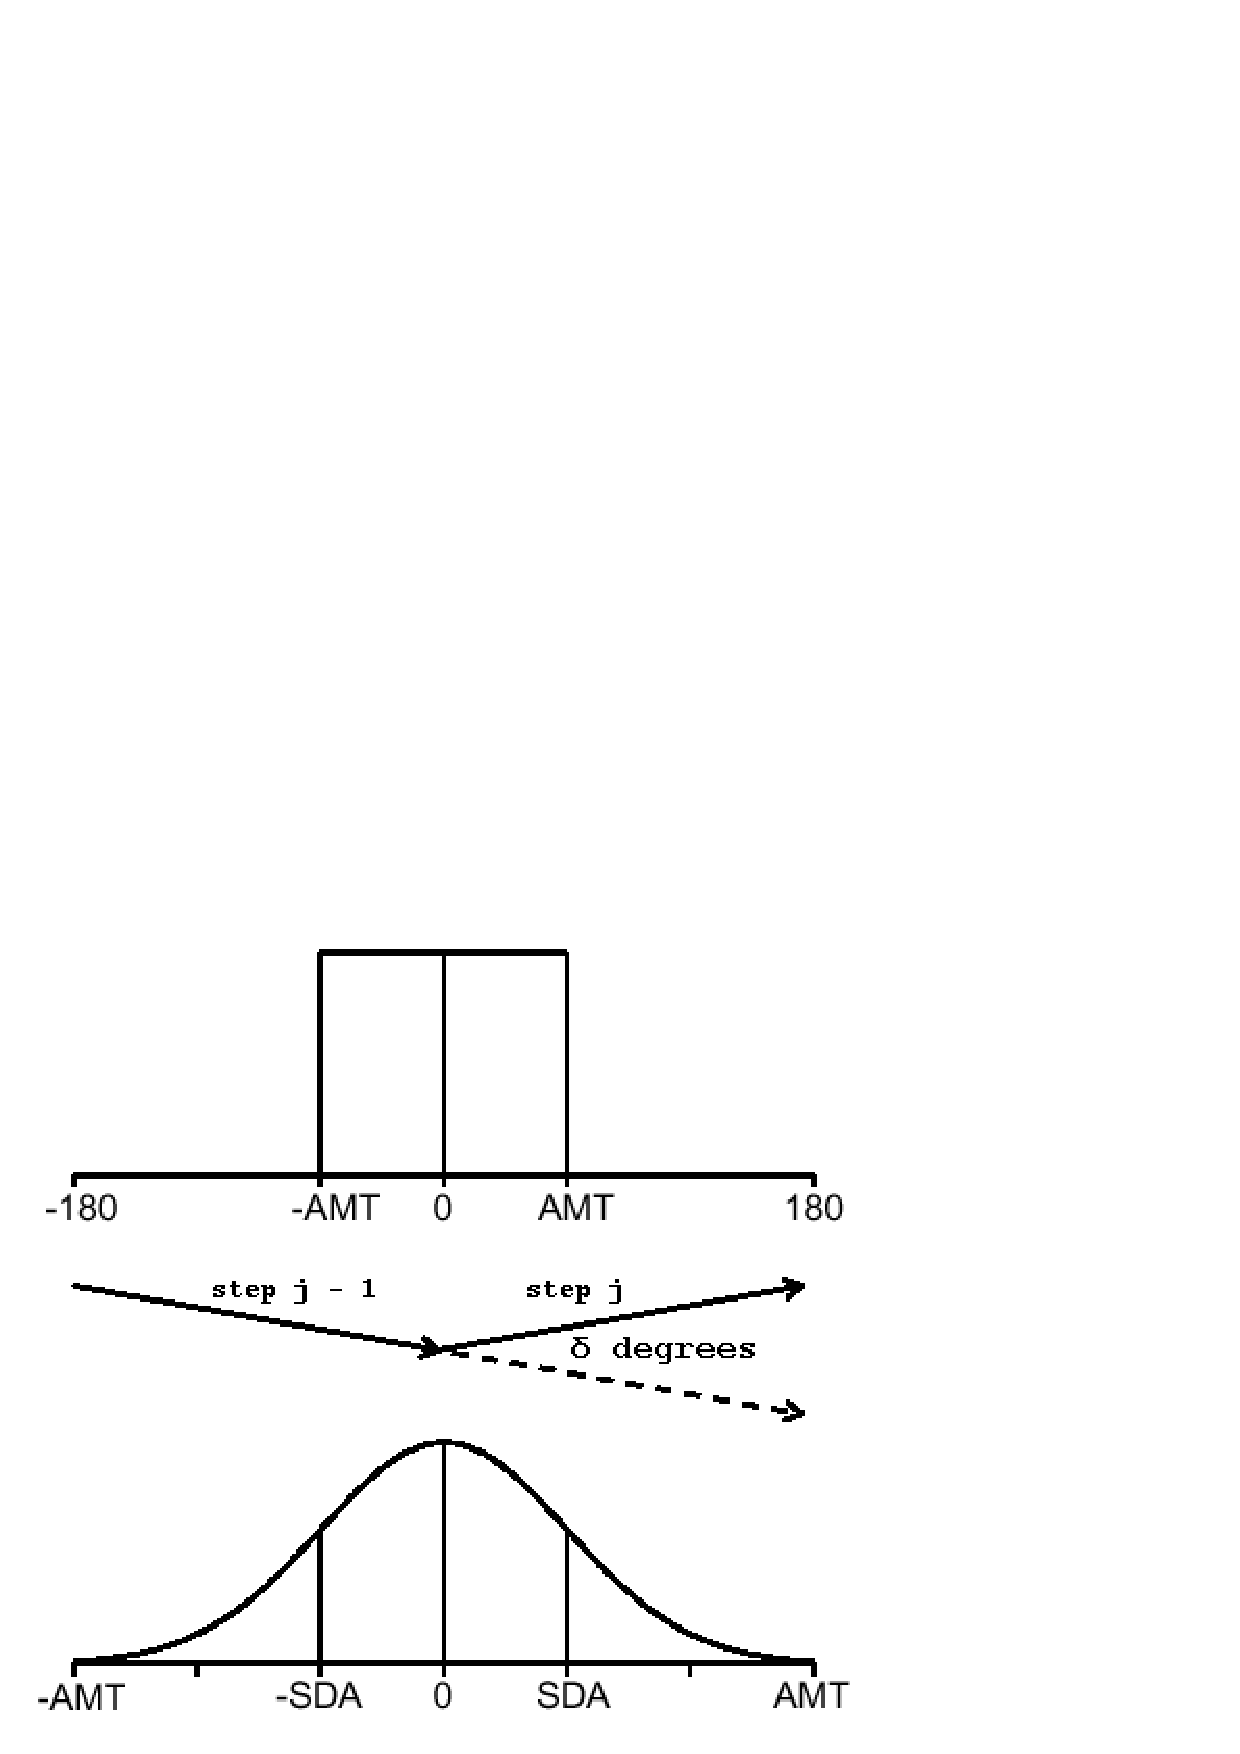
\includegraphics[width=1.0\textwidth]{TADistribution.pdf}
    \end{center}
    \caption{Turning Angle for (a) uniform distribution and (b) depiction
    of what a path may look like.}
  \end{figure}
  Alternatively, if the animal is already at a plant then the animal picks a random direction
  uniformly and then takes a step of size $r+1.0$.  This will ensure that the animal will not
  immediately return to the same plant on the very next step.

\subsection{\emph{Pollination}}
  When an animal is on a plant, it collects pollen, distributes pollen, and consumes food. Each
  plant contains a number of flowers, $\phi$, from which an animal may obtain pollen. When an animal
  visits a plant it picks up pollen from one or more flowers. The number of flowers from which an
  animal can obtain pollen is determined by the total number of flowers on a plant, the fraction of
  flowers in bloom at any one time ($a$), the number of times ($j$) the plant has previously been
  visited by an animal, and the maximum fraction of flowers available for pollination ($\eta$). The
  formula for the number of total flowers available for visitation during a $k^{th}$ visit to the
  $j^{th}$ plant ($f_{j,k}$) is given by
  \begin{equation}\label{flowers}
    f_{j,k} = \phi \cdot a \cdot \eta^k.
  \end{equation}

  It is assumed that the amount of food eaten and the amount of pollen collected is proportional to
  the number of visited flowers. An animal collects pollen and eats from every flower that it
  visits, and so the amount of pollen collected and the amount of food eaten is proportional to the
  equation (\ref{flowers}). Let $f^{\left(i\right)}_{j,k}$ be the number of flowers visited by the
  $i^{th}$ animal during the $k^{th}$ visit to the $j^{th}$ plant then the amount of polllen/nectar
  in the $i^{th}$ animal's stomach after $m$ plant visits is given by
  \[
    c^{\left(i\right)}_m = \sum_{j=0}^{m} \beta f^{\left(i\right)}_{j,k},
  \]
  where $\beta$ is the proportionallity constant for the amount of pollen collected at a plant.
  Each animal has a maximum amount of food they will ingest, $c_{max}$, at which time they will stop
  search for food and return to their lair. %The total amount of food that an animal can eat is
  limited
%by the stomach size, $c_{max}$.

  The fraction, $\alpha$, of all flowers are pollinated, and the associated probability that a
  flower is pollinated, $\rho$, are related by the equation,
  \begin{equation} \label{Prob}
    \alpha = \rho \cdot \hat{f}_k.
  \end{equation}
  Using equation (\ref{limit}) and (\ref{Prob}) we can determine the probability that a flower is
  pollinated, $\rho$, by the formula
  \[
    \rho = \frac{\alpha}{\phi} \cdot \frac{1 - \eta}{a \cdot \eta}.
  \]

  When a flower is pollinated it must determined which previous plant donated the pollen. Each
  flower visited is recorded and is available to pollinate the current flower, except those flowers
  that are on the same plant. Self- pollination, is not considered, because the likelyhood of
  self-pollination is low due to mechanisms that impedes self-pollination. Each flower considered
  has an equal likelihood of pollinating the current flower.

\subsection{Time and Stopping Criteria}
  The velocity an animal travels ($v$) is assumed to be constant, as well as the time spent on a
  plant ($t_{plant}$).  The travel time for an animal is then given by the formula
  \[
    t^{\left(i\right)} = \frac{s^{\left(i\right)}}{v} + T^{\left(i\right)} \cdot t_{plant},
  \]
  where $T^{\left(i\right)}$ is the number of plants visited by the $i^{th}$ animal. If we let the
  maximum allowable travel time be $t_{max}$, then once $t^{\left(i\right)} \geq t_{max}$ or
  $c^{\left(i\right)}_m \geq c_{max}$ the animal is removed from the simulation. $t_{max}$ is based
  on the optimal searching time during the day.  When there are no animals left the simulation
  terminates.

\subsection{Model Statistics}

  To best explore the inherent differences between biotic and abiotic pollination this study focuses
  on the effects of movement as well as the effects of plant density.  
  \begin{table}[h]\label{eqn}
    \begin{tabular}{|l|l|}
      \hline
      % after \\: \hline or \cline{col1-col2} \cline{col3-col4} ...
      Measure & Equation \\ \hline   \hline
      Average Path Distance & $\displaystyle\bar{s} = \frac{1}{b} \sum_{i=1}^b \sum_{j=1}^n s^{\left(i\right)}_j$ \\ \hline
      Average Maximum Distance & $\displaystyle \bar{M} = \frac{1}{b} \sum_{i=1}^b \max_j \sqrt{\left(x^{\left(i\right)}_{1,0}
    - x^{\left(i\right)}_{1,j}\right)^2 +
          \left(x^{\left(i\right)}_{2,0} -
    x^{\left(i\right)}_{2,j}\right)^2}  $ \\  \hline
      Average Pollination Distance & $\displaystyle \bar{p} = \frac{1}{n} \sum_{i=1}^{n} \left(
    \frac{1}{\tau^{\left(i\right)}} \sum_{j=1}^{\tau^{\left(i\right)}}
    \sqrt{\left(x^{\left(i\right)}_1 -
    x^{\left(j\right)}_1\right)^2 + \left(x^{\left(i\right)}_2 -
        x^{\left(j\right)}_2\right)^2}
        \right)  $ \\  \hline
      Average Maximum Pollination Distance & $\displaystyle \bar{P} = \frac{1}{n} \sum_{i=1}^{n} \max_j \sqrt{\left(x^{\left(i\right)}_1 -
    x^{\left(j\right)}_1\right)^2 + \left(x^{\left(i\right)}_2 -
        x^{\left(j\right)}_2\right)^2}$ \\  \hline
      Average Weighted Diversity of Fathers & $\displaystyle E = \frac{1}{n} \sum_{i=1}^n 1/\frac{1}{\left(\tau^{\left(i\right)}\right)^2}
    \sum_{j=1}^{\Delta\tau^{\left(i\right)}} F^2_{j,i} $ \\
      \hline
    \end{tabular}
    \caption{Equations}
  \end{table}
  In order to quantify these differences we measure statistics that are inherent of the animals:
  \emph{Average Path Distance}, \emph{Average Maximum Distance}, and those of the plant:
  \emph{Average Pollination Distance}, \emph{Average Maximum Pollination Distance}, \emph{Average
  Weighted Diversity of Fathers}.  The calculations of these statistics are given in the Table
  \ref{eqn}.

  In these equations it is assumed that $b$ is the total number of animals, $n$ is the total number
  of plants, $(x_{1,0}^{(i)},x_{2,0}^{(i)})$ is the starting location of the $i^{th}$ animal,
  $(x_{1,j}^{(i)},x_{2,j}^{(i)})$ is the location of the $i^{th}$ animal after $j$ steps,
  $\tau^{(i)}$ is the total number of seeds for the $i^{th}$ plant, $\Delta\tau^{(i)}$ is the number
  of different fathers contributing pollen to the $i^{th}$ plant, and $F_{j,i}$ is the number of
  times the $j^{th}$ father contributed pollen to the $i^{th}$ plant.


\section{Results}
  The following results are based on simulations of the model with parameter
values given in \cref{tab:parameter}. %{\bf (Erich do you remember how we chose
%these numbers?)}\textcolor{red}{No, but clearly some of these need some
%justification. I am guessing a got it from one of the references. I have no
%library access, so it is difficult for me to check the references.}
The grid
size was 101 patches by 101 patches.  The standard error was calculated by
dividing the sample standard deviation by the square root of the total number of
samples. The standard errors were all less than 1\% on average, so will not be
shown due to the small size.

\begin{table}
  \centering
  \begin{tabular}{|l|l|l|l|}
    \hline
    Parameter Description & Symbol & Value &  \\ \hline  \label{parameter}
    Total number of animals & b & 1,000 & fixed  \\ \hline
    Maximum time & $t_{max}$ & 1,200 seconds & fixed \\ \hline
    Fraction of blooms at one time & a & 0.2 & fixed \\ \hline
    Maximum fraction of available flowers & $\eta$ & 0.75 & fixed \\ \hline
    Search radius & r & 1.0 & fixed \\ \hline
    Number of flowers per plant & $\phi$ & 100 & fixed \\ \hline
    Probability of pollination   & $\rho$ & 0.4286 & calculated \\ \hline
    Number of plants & n & 1000 & fixed \\ \hline
    Time spent at each plant & $t_{plant}$ & 100 seconds & fixed \\ \hline
  \end{tabular}
  \caption{Parameter Values}
  \label{tab:parameter}
\end{table}

\begin{figure}
  \begin{center}
  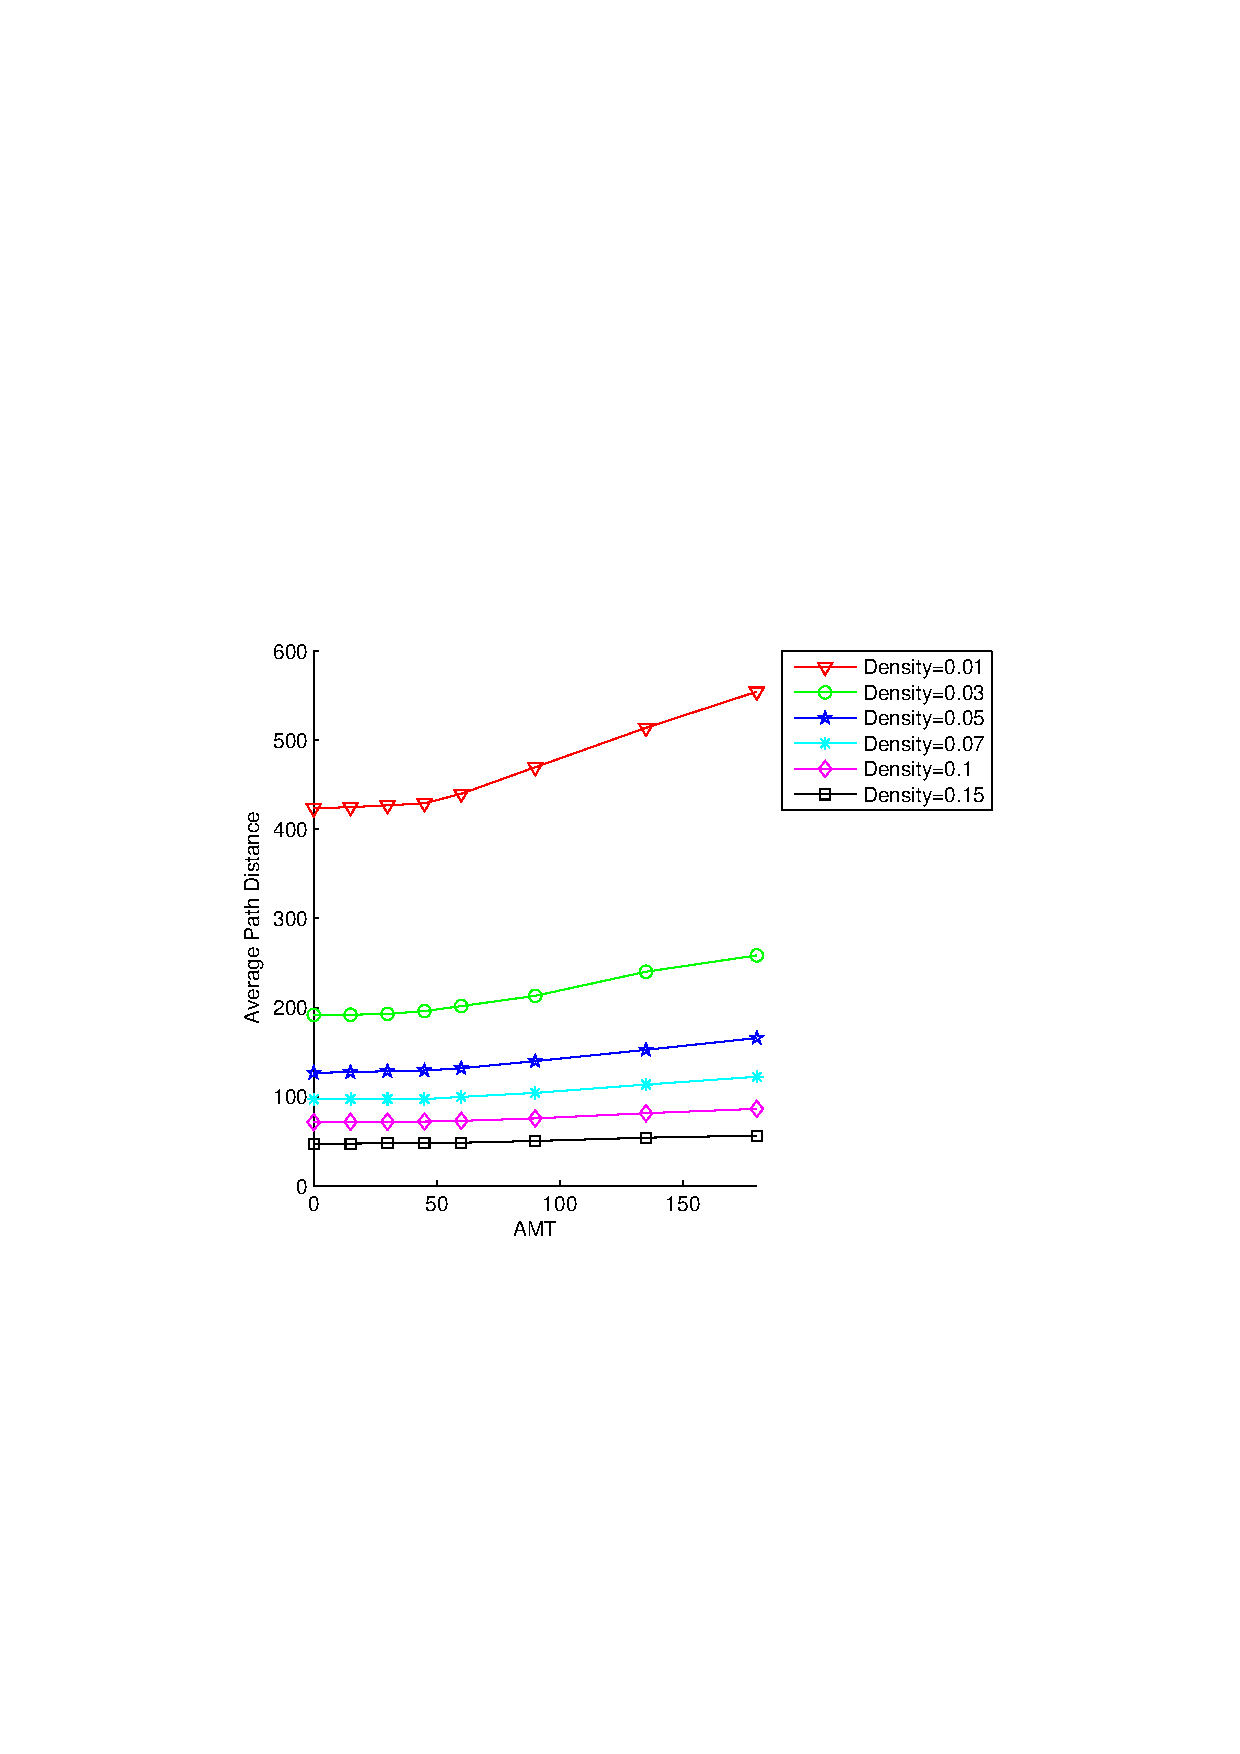
\includegraphics[scale=0.5]{Figures/PathVsAMT.pdf}
  \end{center}
  \caption{\small Average Path Distance vs. Turning Angle for Various Plant
    Densities}
  \label{AvgPathN}
\end{figure}

In \cref{AvgPathN} the average distance traveled for each animal decreases
with increasing density due to higher foraging success.  In this situation the
animals will spend more time on plants since they can find plants more readily
and thus reach their maximum searching time more quickly.  The maximum turning
angle does not have a large effect on on the  average distance in general,
though there is a modest effect at low plant densities where the larger values
increase the average distance due to less success at foraging.

On the other hand, the average maximum distance traveled by animals, see
\cref{AvgMaxDBees}, is affected by both the turning angle and plant density.
As with the average path distance, the maximum distance decreases with higher
density for the same reason that this decreases the overall travel time for the
animals since they spend more time on plants.  In this case due to the movement
patterns the maximum turning angle has a large effect on maximum distance
traveled especially at lower densities.  As the maximum angle decreases the
animals are moving in a more highly correlated random walk and are more likely
to travel directly away from their starting points increasing the maximum
distance traveled.

In particular at high density for a moderately correlated random walk
$(AMT=90^{\circ})$ there is an increase of over 30\% for the maximum distance
over the purely random walk, and for a highly correlated random walk
$(AMT=45^{\circ})$ there is an increase of 67\%.  At lower densities this is
more pronounced.  There is an increase in the maximum distance traveled by 62\%
and 160\% over the purely random walk by a moderately and highly correlated
random walks, respectively. These differences can have important consequences on
the overall genetic diversity for the plants, and shows that biotic dispersal
has a greater potential for long range pollination over abiotic
dispersal.

\begin{figure}
  \begin{center}
  \includegraphics[scale=0.5]{Figures/MaxDVsAMT.pdf}
  \end{center}
  \caption{\small Average Maximum Distance vs. Turning Angle for Various Plant Densities}
  \label{AvgMaxDBees}
\end{figure}

We see this potential in \cref{AvgDist} where, like the average maximum
distance, the average pollination distance increases with stronger correlation
and at lower density.  At high densities the effects of correlation are smaller.
This is due to the fact that when pollinators plants they leave each
plant in a random direction, and so as plant density increases the number of
plant visits increases, which consequently has them behave more like a
purely random walk.  It is also the case, as with the average maximum distance,
as the maximum angle decreases and the correlation strengthens, the animal is
likely to travel farther from its initial position, which allows for longer
pollination distances.

At low densities there is an increase in the average pollination distance of
36\% and 96\% over a purely random walk for a moderately and highly correlated
random walk, respectively.  At high density the increases are 29\% and 65\%,
respectively.  These increases will have significant impact on the overall gene
flow of the plant species.

\begin{figure}
  \begin{center}
  \includegraphics[scale=0.5]{Figures/PollenDVsAMT.pdf}
  \end{center}
  \caption{\small Average Pollination Distance vs. Turning Angle for Various Plant Densities}
  \label{AvgDist}
\end{figure}

These increases are also observed for the maximum pollination distance.  For low
plant densities the average maximum pollination distance increases by 53\% for
moderately correlated random walks over purely random walks, and 148\% for
highly correlated random walks.  Additionally, for high plant densities these
increases are 44\% and 96\% for moderately and highly correlated random walks
over purely random walks, respectively.  Since these are average values there is
clearly a potential for much greater range of pollen dispersal and genetic
variation with biotic dispersal over abiotic dispersal.

\begin{figure}
  \begin{center}
  \includegraphics[scale=0.5]{Figures/MaxPollenVsAMT.pdf}
  \end{center}
  \caption{\small Average Maximum Pollination Distance vs. Turning Angle for Various Plant Densities}
  \label{AvgMaxDTreesN}
\end{figure}

Plant density affects the maximum pollination distance in a more complex
fashion.  The higher the density the more gradual the decrease is in the maximum
pollination distance as the maximum turning angle increases.  Whereas, at lower
densities this decrease is much larger.  This is due to the fact at lower
densities pollination occurs less frequently with a larger variability of
maximum pollination distances.

\begin{figure}
  \begin{center}
  \includegraphics[scale=0.5]{Figures/WDFvsAMT.pdf}
  \end{center}
  \caption{\small Average Weighted Diversity of Fathers vs. Turning Angle for Various Plant Densities}
  \label{EFathers}
\end{figure}

In general there is a small decrease in the average weighted diversity of
fathers as the maximum turning angle increases, see \cref{EFathers}. With
higher maximum turning angles the search patterns tend to be more circular
lowering the overall diversity that a plant will see since pollinators will
visit the same plants more frequently.  On the other hand, by increasing the
density, plants will see an increase in diversity due to the larger amount of
plants near by.  This increase lessens at higher densities due to the limited
foraging time of the pollinators.

\section{Discussion}
  Pollination is a critical process to all life and is a very difficult one to study for a variety of reasons: pollen size, pollinator diversity, plant diversity, etc.  In this study we have used a single agent-based model with correlated random walk to simulate both abiotic and biotic pollination.
This simulation approach provides a powerful method for studying pollination given the logistical difficulties associated with direct field monitoring.
  
A striking result is increases in pollination distances, average and maximum, that occur with the biotic model versus the abiotic model.  In particular at both low and high densities we observe at least 29\% and as high as 96\% increases in the average distance pollen travels in moderately or highly correlated random walks over the purely random walks.  For the average maximum pollination distance the increases range from 44\% to 148\%.  This can lead to unexpected consequences especially if say an animal pollinated, genetically modified crop is placed a particular distance from an non-genetically modified crop based on a purely random diffusion model.  In this situation there could be unintended cross contamination.


The majority of models studying pollination have assumed a purely random diffusion process. There is
clear evidence that there are differences in statistics seen between plants pollinated through wind
dispersal from those pollinated through animal dispersal \cite{LevinKerster}.  We demonstrate here how large these differences can be.
{\bf Add some important biology language on the consequences of these observations.}

It is clear from the results that density plays a large role in the overall gene flow for a species.  However in most of the statistics we calculated how animals move is also very important.  Generally the statistics are affected by movement more at low densities and less so at high densities.
%As can be seen in the results section the magnitude of turning angle had varying degrees of effects
%over different plant densities and therefore pollination patterns predicted by a model assuming a
%purely random walk could be vastly different from a model assuming a correlated random walk.
%For
%high plant densities, the effects of correlated random walk was less pronounced than that of low
%plant densities, except for the \emph{average weighted diversity of fathers}. In the case of
%\emph{average weighted diversity of fathers} the affect of turning angle magnitudes were more
%pronounced for high densities. Therefore, although diffusion models for densely populated plant
%species may not vary greatly from models that assume a correlated random walk for \emph{average
%pollination distance} or \emph{average maximum pollination distance} they will vary significantly
%for \emph{average weighted diversity of fathers}. This has the affect of under estimating the
%diversity of pollination for high plant densities and animal dispersal as compared to similar plant
%densities and wind dispersal.

%The variation between correlated random walk and that of a purely random walk is significant at low
%plant densities for the statistics such as \emph{average maximum distance}, \emph{average
%pollination distance}, and \emph{average maximum pollination distance} and so for the case of low
%plant densities the assumption of a purely random walk may lend to bias in the analysis of
%pollination. Most studies to date have been conducted on small herbaceous plant species whose
%densities tend to be high. Even though most of the animals statistics presented were not greatly
%influenced by turning angle for high plant densities the average weighted diversity of fathers had was
%still greatly affected by the turning angle at these densities, and therefore an assumption of a
%purely random walk would be an inappropriate assumption and at any of the densities examined in this
%study. Therefore a correlated random walk may be a better approximation to animal movement.




\subsection*{Acknowledgments}
This work was performed as a component of the Masters degree for ELF.  Portions of this research were supported by a National Science Foundation grant (DEB-0640803) to RJD and DMC.  The authors would like to thank \emph{who helped out here?  Anyone of consequence?}

\bibliographystyle{amsplain}
\bibliography{PollenPaper}%xbib}
\end{document}
